%%% Local Variables:
%%% mode: LaTeX
%%% TeX-master: t
%%% End:

\documentclass{beamer}
\usepackage[utf8]{inputenc}

\usetheme{Berkeley}

%\useoutertheme{shadow}
%\useinnertheme{rounded}

\definecolor{BSUblue}{RGB}{0, 51, 160} % (primary)
\definecolor{BSUorange}{RGB}{214,67, 9} % (secondary)

\setbeamercolor{palette primary}{bg=BSUblue,fg=white}
\setbeamercolor{palette secondary}{bg=BSUblue,fg=white}
\setbeamercolor{palette tertiary}{bg=BSUblue,fg=white}
\setbeamercolor{palette quaternary}{bg=BSUblue,fg=white}
\setbeamercolor{structure}{fg=BSUblue} % itemize, enumerate, etc
\setbeamercolor{section in toc}{fg=BSUblue} % TOC sections

% Override palette coloring with secondary
\setbeamercolor{subsection in head/foot}{bg=BSUorange,fg=white}


%------------------------------------------------------------
%Title page
\title[Rusty Linux] {Rusty Linux: Advances in Rust for Linux Kernel Development}

\author[]
{Shane K. Panter\inst{1} \and Nasir, Eisty\inst{2}}

\institute[BSU]
{
  \inst{1}%
  Clinical Assistant Professor\\
  Boise State University
  \and
  \inst{2}%
  Assistant Professor\\
  Boise State University
}

\date[ESEM 24]
{International Symposium on Empirical Software Engineering and Measurement, October 2024}

\logo{
\includegraphics[height=1cm]{images/bsu-logo.eps}}

%End of title page configuration block
%------------------------------------------------------------


\begin{document}

\frame{\titlepage}

\section{Introduction}
\begin{frame}
  \frametitle{Introduction}
  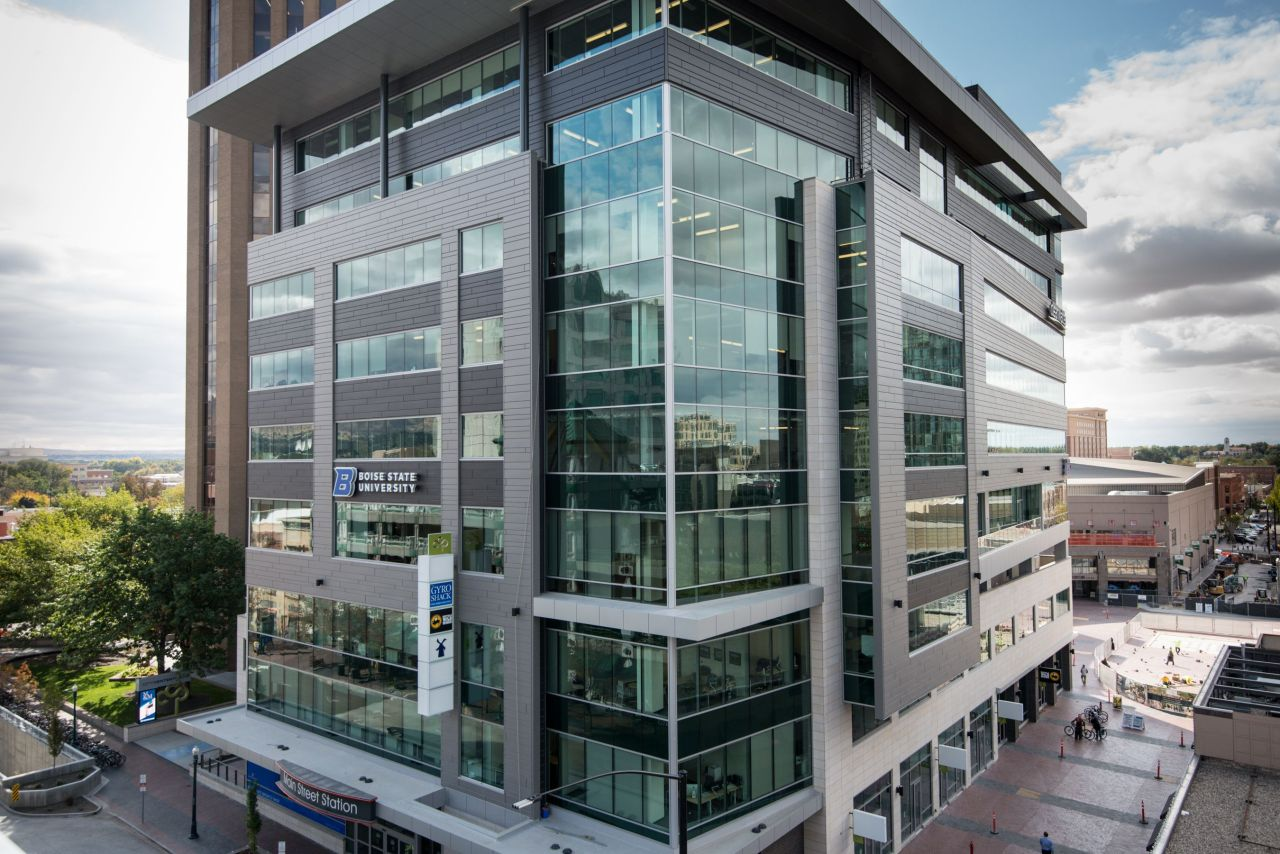
\includegraphics[width=3in]{images/CCP-from-northwest.jpg}
  \begin{block}{Boise State University}
    The Computer Science Department is located in Beautiful downtown Boise Idaho, United States!
  \end{block}

\end{frame}


\section{Methodology}
\begin{frame}
  \frametitle{Process Diagram}
    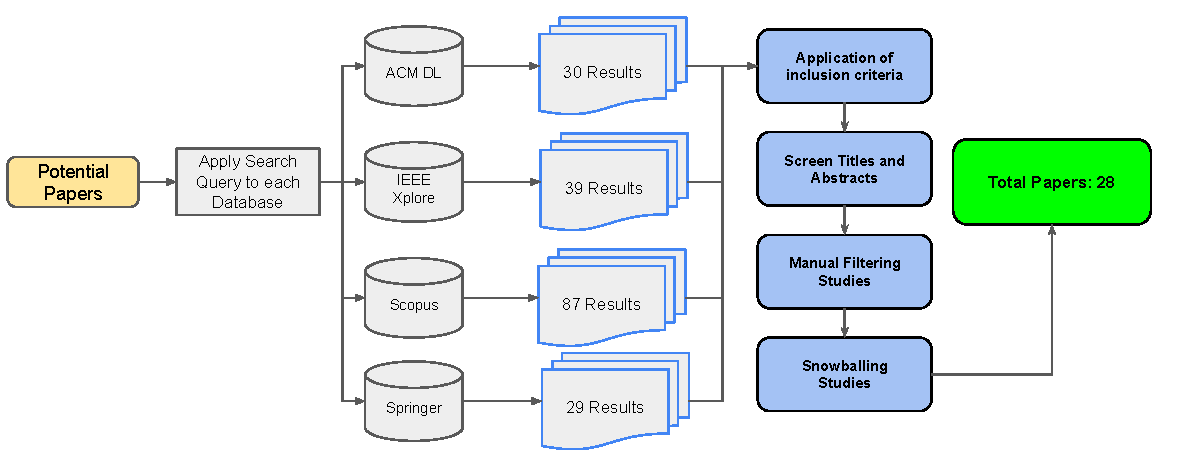
\includegraphics[width=4in]{figures/process-diagram.pdf}
\end{frame}

\section{Results}

\end{document}
